% SPDX-License-Identifier: LPPL-1.3c
% Copyright (C) 2026 Christophe Jorssen
% Author and Current Maintainer: Christophe Jorssen <christophe.jorssen@gmail.com>
% LPPL maintenance status: maintained
% This file is part of luafemm. See LICENSE and LICENSES.md for its terms.
\section{A tutorial: let a conducting screen find its potential}
\label{sec:tutorial-electric-floating}

Kamil now inserts a thin conducting screen between two capacitor plates. The
screen has no wire to a voltage source. Assigning it zero volts would describe
a grounded screen, not the experiment he wants. Instead he specifies that
its total charge is zero and lets the calculation find its potential.

\luafemmexamplebegin{electric-floating}
\subsection{Declare the conductor, then ask for the field}
Kamil starts with a coarse |mesh size=.2|. His cell has insulating horizontal
sides to isolate the simple one-dimensional experiment. The plates are two
centimetres apart and the planar depth is three centimetres. A native TikZ
style collects the floating electrode's physical keys and drawing appearance.

\Needspace{12cm}
\begin{codeexample}[width=0pt]
\tikzset{lesson floating screen/.style={orange!80!black,very thick,
    femm/electric electrode={name=screen,condition=charge}}}
\begin{tikzpicture}[femm/electrostatic={model=finite elements,
    xmin=0,xmax=2,ymin=0,ymax=1,depth=3,
    outer boundary=insulated,mesh size=.2,name=screen cell},scale=1.6]
  \draw[very thick,femm/electric electrode={name=left,potential=10}]
    (0,0)--(0,1);
  \draw[very thick,femm/electric electrode={name=right,potential=0}]
    (2,0)--(2,1);
  \draw[lesson floating screen] (1,0)--(1,1);
  \pic {femm electric field};\pic {femm equipotentials};
  \node[above] at (0,1) {$10$ V};
  \node[above] at (1,1) {$Q=0$};
  \node[above] at (2,1) {$0$ V};
\end{tikzpicture}
\qquad
$V_s=\femmelectricvalue[model=screen cell,electrode=screen,
    quantity=voltage]$ V.
\end{codeexample}

The neutral screen settles at $5$ V. Its two faces carry opposite charges;
zero total charge does not mean zero local surface charge. Field lines terminate
on the screen and continue separately from its other face. For a finite-width
screen, Kamil would enlarge the surrounding dielectric and check mesh and
exterior-boundary sensitivity instead of keeping this ideal cell geometry.

A nonzero |charge| would be supplied in coulombs. Several separated paths can
share |name=screen| if an ideal connecting wire makes them one conductor.
Their prescribed charge is counted once. To repeat an experiment with another
charge, Kamil starts another physical picture: the field pic has already frozen
this model. He only refines the mesh once the geometry and teaching narrative
have settled.

\subsection{Measure the terminal capacitances}
The named snapshot remains available after the picture. Kamil selects only
the two driven electrodes as matrix ports; the floating screen is eliminated
with zero incremental charge. He can ask for a matrix without changing the
$10$ V operating state used by the preceding drawing.

\Needspace{6cm}
\begin{codeexample}[width=0pt]
\femmelectricmatrix[name=screen capacitance,model=screen cell,
    electrodes={left,right}]
$C_{11}=\femmelectricmatrixvalue[matrix=screen capacitance,
    row=left,column=left]$ F,
\quad
$C_{12}=\femmelectricmatrixvalue[matrix=screen capacitance,
    row=left,column=right]$ F.
\end{codeexample}

Here $C_{11}=\epsilon_0 hd/d_{\rm gap}$, where $h=1$ cm is the drawn plate
height, $d=3$ cm the extrusion depth and $d_{\rm gap}=2$ cm the separation.
The off-diagonal coefficient is negative. With all independent charges zero,
$\mathbf Q=C\mathbf V$ and $W=\tfrac12\mathbf V^TC\mathbf V$.
With prescribed charges present, Kamil must also retrieve |quantity=offset charge|;
using $Q/V$ alone would mix the source offset with capacitance.

\subsection{Let PGFPlots present the result}
There is no separate chart language to learn. Kamil uses an ordinary bar axis,
labels its row indices with electrode names, and selects one captured column.

\Needspace{11cm}
\begin{codeexample}[width=0pt]
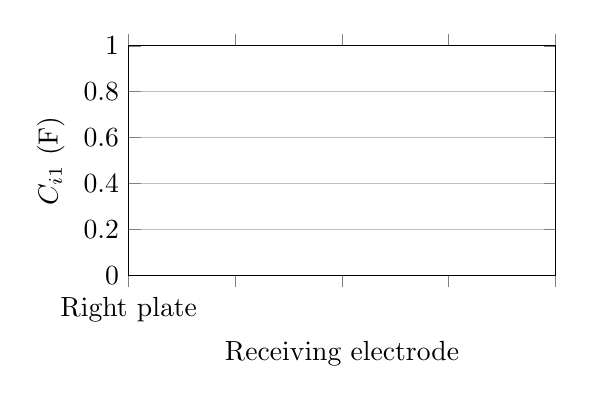
\begin{tikzpicture}
  \begin{axis}[width=7cm,height=4.5cm,ybar,
      xtick={1,2},xticklabels={Left plate,Right plate},
      xlabel={Receiving electrode},ylabel={$C_{i1}$ (F)},
      ymin=-1.8e-13,ymax=1.8e-13,enlarge x limits=.5,
      ymajorgrids,bar width=14pt]
    \femmelectricmatrixplot[matrix=screen capacitance,column=left,
      plot options={fill=blue!30,draw=blue!60!black}]
  \end{axis}
\end{tikzpicture}
\end{codeexample}

For a two-dimensional comparison independent of extrusion depth, Kamil can
capture a second matrix with |normalization=per length| and label its axis
in F/m. That normalization has no meaning for a complete axisymmetric body;
its capacitance is already in farads.
\luafemmexampleend{electric-floating}
